% vim: fo=aw2tq tw=100 spell
\chapter{Testing and Evaluation}
\label{sec:testing}

This section is a commentary on the testing procedures used throughout the project.  My general 
approach was bottom-up iterative development and testing---starting with the most basic components 
that stand on their own, testing them thoroughly, and building the next layer of complexity on top 
of them.  Every component that is tested well and known to be working provides a good stable 
platform for testing other components against.

\section{Output Hardware}
\label{sec:testing:hardware}

Using the principle of testing components with already working components, it made sense that the 
first part that needed to be tested was the audio hardware.

After assembling the audio output hardware as designed (and illustrated in 
Appendix~\ref{appendix:circuit-diagram}), but before connecting the data lines to the parallel I/O 
ports, the behaviour was tested manually by setting input values with 8-bit DIP switches, and 
measuring voltages with an oscilloscope.

First, both inputs were set to the maximum values, and the voltage measured from the output of the 
second op-amp (IC4, pin 6).  This is the maximum voltage.  Starting from the MSB, each bit of the 
input to the volume DAC was switched from ``on'' to ``off'', and the voltage observed at each point.  
The voltage was halved for every bit turned off, as expected.  This showed that the first DAC was 
operating correctly, and that the ``pre-scaling'' effect also worked correctly.

The experiment was repeated, but this time changing only the value of the waveform DAC.  The same 
results were observed, as expected.  This means this DAC was also working correctly.

Next, an 8-bit binary counter was assembled and run as the input to each DAC in turn to test the 
response to changing inputs.  The observed waveform on the oscilloscope revealed overshoot in the 
output when the value changed.  Fixing this issue is described in 
Section~\ref{sec:design:hardware:feedback}.  Other than this, the device performed as expected.

The oscilloscope probe was then moved to the output of the audio amplifier.  Since a binary counter 
provides a sawtooth wave, the previous test was already providing the maximum jump between values.  
We found that if we turned the potentiometer to its maximum value, the top of the wave would be 
clipped, however through most of the range the waveform was correct.


\section{Output Interface}

Testing the software interface to the output device was as simple as writing a simple loop program 
to cycle through a mock waveform, at three different volumes.  I did this for a simple 8-point 
``sine'' wave, which displayed as expected (not anything like a sine wave because of the short 
transition time) --- this also gave me an idea of the maximum rate at which the output device could 
be driven, since there was no delay inserted in the loop.

\section{PRT-Based Playback}

A program was created which used a PRT interrupt to drive the playback.  The interrupt handler 
alternated between 00h and FFh, giving a square wave.  The tests mainly involved obtaining specific 
frequencies by setting the PRT reload register value.

\section{Wavetable Playback}

When I implemented PRT-based wavetable playback, the startup routine of the software involved 
setting the device playing a particular note.  A single 256-sample 2-wave sine wavetable was created 
for testing the software (instrument samples were left till later in the project once everything 
else was working).  The oscilloscope probe was attached to the amplifier output so I could see the 
output waveform and check that it matched what should be output.  Figure~\ref{fig:oscilloscope} 
shows the oscilloscope when playing one of the final instrument samples.

\begin{figure}[htb]
\centering
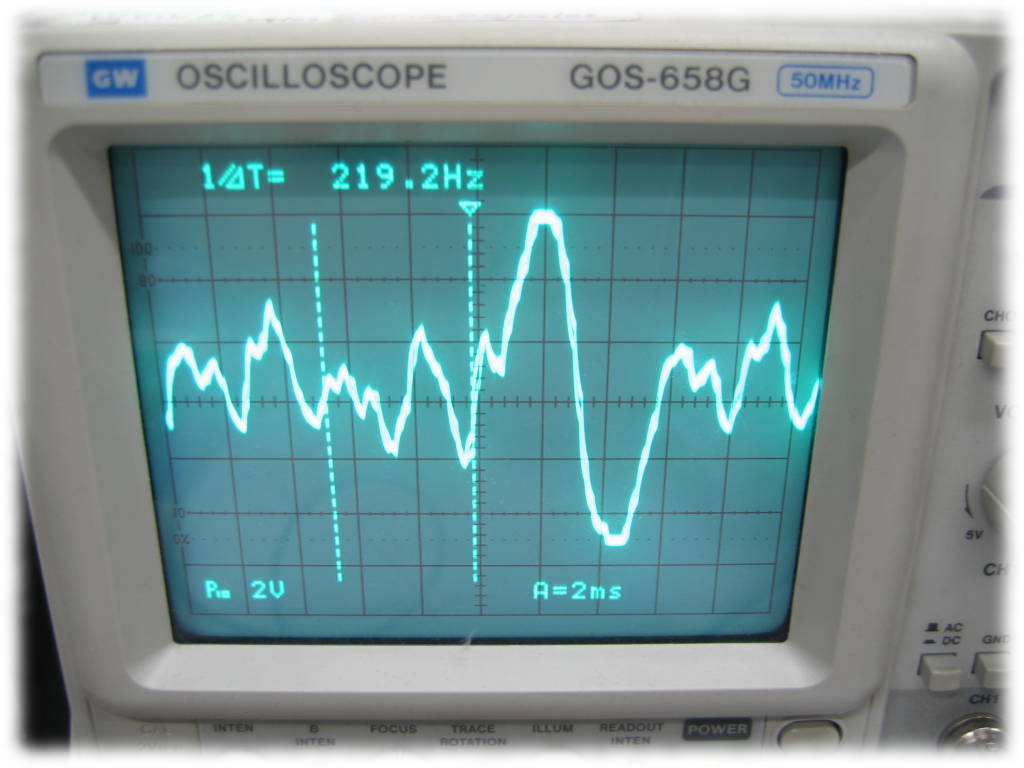
\includegraphics[width=0.7\textwidth]{images/oscilloscope}
\caption{Oscilloscope Trace of Amplifier Output}\label{fig:oscilloscope}
\end{figure}

\section{Terminal Interface}

Testing the terminal interface was a simple matter of echoing back everything sent to the device.  
After this, sending stuff to the terminal could be used as a diagnostic for other parts of the 
software.

\section{Network Interface}

In the first instance, testing the network interface was set up correctly was a matter of echoing 
everything received to the terminal --- this at least verified that something was arriving.

Testing that the correct data was being received was more subjective.  This involved listening to 
the audio output to make sure it sounded right.  The most common error I had which could be heard 
was using the volume data as the note --- this has a very distinctive sound because of the volume 
decay in the network data.

\section{LCD Text Display}

Testing the LCD text display functions I wrote just involved writing some characters to different 
positions on the screen.

\section{Keypad Interface}

Testing the keypad interface was done by making the keypad handler output the value of the key 
pressed to the terminal.
